\chapter{Introduction}\label{cap:intro}

High-performance computing~(HPC) system architectures are getting more
complicated and diversified. Due to the system complexity, performance
optimizations specific to processor architectures, system
configurations, compilers, and/or libraries, called
\emph{system-specific optimizations}, are mandatory and becoming more
important to exploit the potential of a particular system; an
application code must be thoroughly optimized and specialized for one
platform to achieve high performance.  As a result, one HPC application
often needs to have multiple versions, each of which is optimized in a
different way for adapting to a particular platform.  The diversity of
system architectures increases the number of optimized versions required
for performance portability across major platforms.  To make matters
worse, popular platforms can change drastically, and thus an application
might need to be optimized not only for current major platforms but also
for future ones.  Accordingly, an increase in system complexity and
diversity would force a programmer to further invest enormous time and
effort for HPC application development and maintenance.

%The goal of the Xevolver project is to separate system-specific,
%system-aware performance optimizations from application codes.

%XevXML has been developed to express any code modifications separately
%from an application code. Practical HPC application development is a
%team work of multiple programmers.

XevXML is a code transformation framework that allows users to define
their own code transformations, called \emph{user-defined code
transformations}.  It exposes an abstract syntax tree~(AST) to users so
that they can apply any transformations to the AST. Transformation rules
written in external files can be defined for individual systems,
compilers, libraries, and so on.  That is, code transformations
representing system-aware optimizations can be separated from an
application code.  Hence, to achieve high performance, the users no
longer need to specialize an application code for a particular platform.

XevXML assumes that an application code is annotated with a special
mark, using directives and/or comments, and transformations are applied
to the marked parts of the code.  Note that the mark indicates ``where
to transform,'' but does not indicate ``how to transform.''  The
transformation rules that indicate how to transform the code are defined
in external files. If system-aware code modifications are expressed as
code transformations, users can express system-awareness separately from
an application code.

As the name implies, XevXML employs eXtensible Markup Language~(XML) to
represent an AST, i.e.,~an internal representation of code structures
used by compilers.  XML is a widely-used data format, and various
XML-related technologies and tools have already been standardized and
matured.  Therefore, the users implement special code transformations by
using only those standard tools.  This chapter briefly describes an
overview of code transformation with XevXML.

\section{An overview of XevXML}
\begin{figure}[htb]
 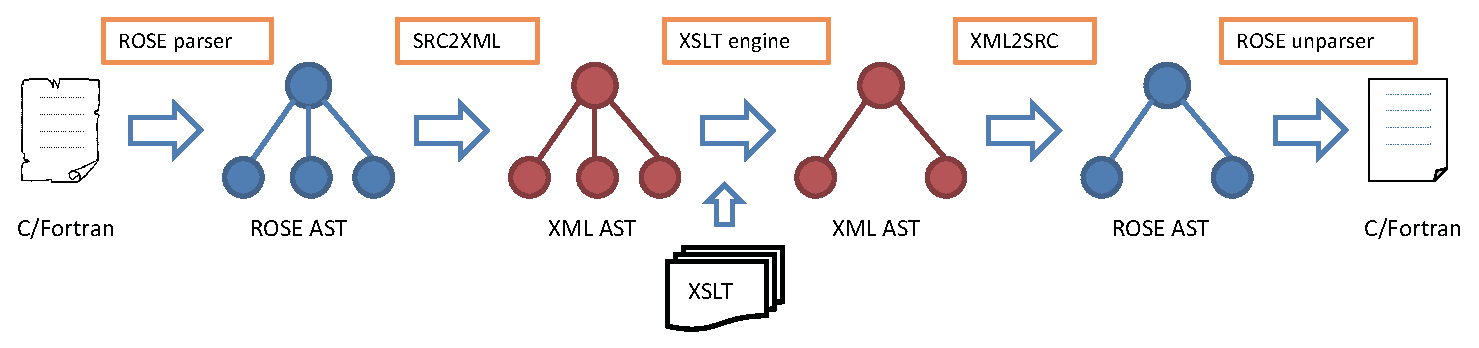
\includegraphics[width=\textwidth]{overview.eps}
 \caption{An overview of interconversion between ROSE ASTs and XML
 ASTs.}\label{fig:overview}
\end{figure}

XevXML has so far been developed on top of the ROSE compiler
infrastructure~\cite{rose}.  XevXML provides the interconversion between
an ROSE AST and its XML representation. Figure~\ref{fig:overview} shows
an overview of the interconversion.  XevXML converts a ROSE AST to an
XML representation of the AST, called an \emph{XML AST}. In XevXML, an
XML AST is exposed to users.  After user-defined transformations, the
transformed XML AST is again converted back to a ROSE AST so that ROSE
can unparse it to a C or Fortran code.

The interconversion is achieved by combining the following two commands,
\texttt{src2xml} and \texttt{xml2src}.

\begin{framed}
\begin{description}
 \item[NAME]~\\
	    \texttt{src2xml} -- source-to-xml translator

 \item[SYNOPSIS]~\\
	    \texttt{src2xml [OPTIONS] INPUT-FILE}

 \item[DESCRIPTION]~\\ \texttt{src2xml} converts a C or Fortran code
	    into an XML document. \texttt{src2xml} reads a code from the
	    input file given by the command-line argument, and prints
	    an output XML document to the standard
	    output. \texttt{src2xml} also accepts some of ROSE
	    command-line options such as \texttt{-rose:verbose}. A ROSE
	    command-line option \texttt{-rose:skip\_syntax\_check} is
	    automatically appended to the command-line options because
	    it is required for some Fortran90 codes.

 \item[EXAMPLES]~\\ \texttt{src2xml hello.c $>$ hello.xml}\\ This command
	    will read \texttt{hello.c} and output its AST as an XML
	    document to \texttt{hello.xml}.
\end{description}
\end{framed}

\begin{framed}
\begin{description}
 \item[NAME]~\\
	    \texttt{xml2src} -- xml-to-source translator

 \item[SYNOPSIS]~\\
	    \texttt{xml2src [OPTIONS]}

 \item[DESCRIPTION]~\\ \texttt{xml2src} converts an XML AST to a C or
	    Fortran code. Since the original language, C or Fortran, is
	    recorded in an XML AST, \texttt{xml2src} generates a code
	    written in the original language. \texttt{xml2xml} reads an
	    XML AST from the standard input, and prints the generated
	    code to the standard output. At present, command-line
	    options for \texttt{xml2src} are simply ignored.

 \item[EXAMPLES]~\\ \texttt{xml2src $<$ hello.xml $>$ hello-again.c}\\
	    This command will read \texttt{hello.xml} and output its
	    code to \texttt{hello-again.c}.
\end{description}
\end{framed}

An XML AST is exposed to users. Thus, the users can apply any
transformation to the AST. As an AST is represented as an XML document,
any XML-related technologies and tools are available for the
transformations. XevXML employs XML Stylesheet Language
Transformation~(XSLT) as the low-level interface to express the
transformation rules of an XML AST.  AST transformation is what
compilers do internally for code transformation. Therefore, XevXML is
capable of implementing various code transformations.

XevXML can easily collaborate with ROSE.  ROSE already has various
features of code analyses and transformations to implement custom code
transformation programs in C++.  It must be painful if a user is
required to reimplement those features from scratch for XevXML. So
XevXML provides not only the above basic commands but also some C++
classes and functions, which are helpful to read and write XML ASTs, so
that code transformation programs developed with ROSE can handle XML
ASTs. Those classes and functions will be further described in
Chapter~\ref{chap:internal}.

If a code transformation is general enough and hence reusable in many
applications, it could be implemented using either ROSE or XevXML.
However, code transformations in practice could be application-specific,
system-specific, domain-specific, and even programmer-specific. If such
a code transformation program is implemented with ROSE, the user needs
to maintain the program in addition to his/her application code. In
XevXML, only transformation rules are defined declaratively, and code
transformations are performed using standard XML tools. So the user does
not need to develop his/her own program for applying the rules to
application codes.

%XevXML needs to be flexible enough to express various code
%transformations required in practical performance optimizations.

%If the user is familiar with ROSE, he/she can develop a code
%transformation by using ROSE.

%and write the result as an XML document.



\section{XML elements and attributes}\label{sec:xml}
Let's get started with a simple example, ``Hello, World!'' in C.
\begin{framed}
\begin{src}
#include <stdio.h>

int main()
{
  printf("Hello, World!\n");
  return 0;
}
\end{src}
\end{framed}


Using the \texttt{src2xml} command, the above code is converted to an
AST of the following XML document.

\begin{framed}
\begin{src}
<?xml version="1.0" encoding="UTF-8"?>
<SgSourceFile filename="hello.c" language="2" format="2">
  <SgGlobal>
    <SgFunctionDeclaration name="main"  end_name="0" >
        <SgTypeInt/>
      <SgFunctionParameterList/>
      <SgFunctionDefinition>
        <SgBasicBlock>
          <SgExprStatement>
            <SgFunctionCallExp>
              <SgFunctionRefExp symbol="printf" />
              <SgExprListExp>
                <SgCastExp mode="0" >
                    <SgPointerType base_type="SgModifierType" >
                      <SgModifierType modifier="const" >
                        <SgTypeChar/>
                      </SgModifierType>
                      <SgTypeChar/>
                    </SgPointerType>
                  <SgStringVal value="Hello, World!\n" paren="1"/>
                </SgCastExp>
              </SgExprListExp>
            </SgFunctionCallExp>
          </SgExprStatement>
          <SgReturnStmt>
            <SgIntVal value="0"  string="0" />
          </SgReturnStmt>
        </SgBasicBlock>
      </SgFunctionDefinition>
<PreprocessingInfo pos="2"  type="6" >
#include &lt;stdio.h&gt;

</PreprocessingInfo>
    </SgFunctionDeclaration>
  </SgGlobal>
</SgSourceFile>
\end{src}
\end{framed}

The data format of XML ASTs is designed so that the interconversion
between ROSE ASTs and XML ASTs becomes simple.  In general, an XML
document consists of XML elements and their attributes. In an XML AST,
each XML element corresponds to a ROSE AST node. XML attributes of an
XML element are used to keep the necessary information to restore the
ROSE AST node.  An XML AST looks like a text representation of a ROSE
AST.  In other words, XevXML provides another interface, XML, to handle
ROSE AST nodes.

In the above XML document, the first line just indicates that the file
is written in XML.  The root node of an AST is the \texttt{SgSourceFile}
element in the second line. The \texttt{SgSourceFile} element represents
the whole C code.  The \texttt{SgGlobal} element in the third line is a
child node of the root node, and indicates the global scope of the C
code. In the global scope, the \texttt{main} function is declared and
defined. In the function body, the first statement is an expression
statement, and the second statement is a \texttt{return}
statement. Comments and preprocessor information such as
\texttt{\#include $<$stdio.h$>$} are written as strings within the
\texttt{PreprocessingInfo} element.

XML attributes are used to restore ROSE AST nodes. For example, the
\texttt{SgStringVal} element corresponds to a ROSE AST node of a
\texttt{SgStringVal} class object representing a string.  Thus, a string
of \texttt{"Hello, World!$\backslash{}$n"} is written as its
\texttt{value} attribute. Similarly, the \texttt{SgFunctionRefExp}
element is a reference to the name of a function, and the function name
is given as the \texttt{name} attribute. Let's change ``printf'' is to
``puts'' by a text editor. Then, when the modified XML AST is converted
to a C code (by using the \texttt{xml2src} command), the function call
of \texttt{printf} will be changed to that of \texttt{puts}. This is a
simple example to show that, in XevXML, XML data transformation results
in AST transformation and thereby code transformation.

See the ROSE reference manual~\cite{rosemanual} to learn more about the
definition of each AST node.

\section{XML data transformation}\label{sec:xslt}

XML data are texts, and various tools are thus available to modify an
XML AST.  As shown in Section~\ref{sec:xml}, even a text editor can
modify an XML AST.  One may consider that, in the case of using a text
editor, modifying a C/Fortran code is much easier than modifying its XML
AST. So why don't we directly modify the code?  The answer is to avoid
specializing the code for a particular platform.

In many cases, system-aware code optimizations assuming a particular
target platform are necessary to exploit the system performance.  A
problem is that those optimizations are often harmful to the performance
of another platform.  A pragmatic approach is to maintain multiple
versions of a code, each of which is optimized for a different
platform. However, this results in degrading the maintainability and
making legacy application migration more painful.

%The modified AST can be converted back to a C or Fortran code.

XevXML has been developed to replace code modifications with
``mechanical transformations'' of an XML AST.  There are several
benefits of the replacement.  One important benefit is that the original
code is not necessarily specialized for a particular platform.  In other
words, system-awareness is separated from an application code.  This
will be helpful to avoid maintaining multiple versions of an application
code.

Another benefit is that expert knowledge about performance optimizations
can be expressed in a machine-usable way.  Basically, performance
optimizations are very intellectual tasks that are often done on a
case-by-case basis.  However, focusing on a particular case, there are
repetitive patterns in code modifications for performance
optimizations. Thus, the code modifications can be replaced with a
smaller number of mechanical code transformations.

The mechanical code transformations required instead of code
modifications could be application-specific, system-specific,
domain-specific, and even programmer-specific. Thus custom code
transformations are often needed for special demands of individual
cases.  Therefore, XevXML has been developed for users to define their
own code transformations in an easy way.

In XevXML, XSLT is currently employed to describe custom transformation
rules of XML ASTs at the lowest abstraction level\footnote{Several
high-level interfaces for definition of code transformation rules are
also under active development in the Xevolver project.  One of such
interfaces will be described in Chapter~\ref{chap:json}.}  In XSLT, XML
data transformations are themselves written in XML.  XSLT uses XPath
expressions~\cite{xpath} to define a pattern within a tree of XML
elements and attributes.  During the transformation process of XSLT,
every XML element is visited in a depth-first manner.  When a pattern is
found at an XML element, the XML element is altered based on the rule
associated with the pattern.

A simple XPath expression looks like a UNIX file path. In a UNIX file
system, files and directories organize a tree structure. A file path is
a text string to specify a location in the directory tree.  There are
two ways to point to the location of a file or a diretory.  One is an
absolute path, and the other is a relative path.  If the string of a
path starts with \texttt{/}, the path is an absolute path, otherwise it
is a relative path. An absolute path is the path to a file or a
directory from the root diretory. For example, the root directory is
expressed by \texttt{/}, its sub-directory named ``sub'' is expressed by
\texttt{/sub}, and a file named ``xfile'' that is located in the ``sub''
directory is expressed by \texttt{/sub/xfile}.  Note that \texttt{/}
represents the root directory and is also used as a delimiting
character.  On the other hand, a relative path indicates the path from
the working directory where a user or an application is located. When
the working diretory is \texttt{/sub}, a relative path to a
\texttt{xfile} can be represented as \texttt{xfile}, \texttt{./xfile},
\texttt{../sub/xfile}, etc.  Of course, those relative paths point to
the same location because \texttt{.} and \texttt{..} denote the working
diretory and its parent directory, respectively.

As well as a UNIX file path, an XPath expression also points to a
location in an XML document.  For example, the root of an XML document
is denoted by \texttt{/}.  A pattern in XML data is described by a
combination of XPath expressions.


An example of XSLT rules for AST transformation are as follows.
\begin{framed}
\begin{src}
<?xml version="1.0" encoding="UTF-8"?>
<xsl:stylesheet version="1.0"
   xmlns:xsl="http://www.w3.org/1999/XSL/Transform"
   xmlns:exslt="http://exslt.org/common">

  <xsl:template match="/">
    <xsl:apply-templates/>
  </xsl:template>

  <xsl:template match="*">
    <xsl:copy>
      <xsl:copy-of select="@*"/>
      <xsl:apply-templates/>
    </xsl:copy>
  </xsl:template>

  <xsl:template match="SgForStatement">
    <xsl:if test=".//*=SgForStatement">
    startLoopNest(); /* inserted */
    </xsl:if>
    <xsl:copy>
      <xsl:copy-of select="@*"/>
      <xsl:apply-templates/>
    </xsl:copy>
    <xsl:if test=".//*=SgForStatement">
    endLoopNest(); /* inserted */
    </xsl:if>
  </xsl:template>
</xsl:stylesheet>
\end{src}
\end{framed}
The above XML file defines three rules, each of which is described
within the \texttt{xsl:template} element. Based on these rules, an XML
document is transformed to another XML document, called an output XML
document.

The first rule matches the root of an XML document. The rule just
invokes \texttt{$<$xsl::apply-templates/$>$} that by default dictates to
visit all the sub-nodes and apply appropriate rules to them.

The second rule matches every XML element of an XML document, because
its XPath expression is given by a wild-card operator, \texttt{*}. The
rule is applied to an element unless a more specific rule matches the
element.  This rule simply copies the element and its attributes to the
output XML document.  The rule is recursively invoked because it invokes
\texttt{$<$xsl::apply-templates/$>$}.

The third rule matches only an \texttt{SgForStatement} element. It
checks if another \texttt{SgForStatement} element exists in the subtree
of the matched element.  Only if it exists, text data are inserted
before and after the matched element.

If the above XSLT rules are applied to an XML AST, two function calls,
\texttt{startLoopNest()} and \texttt{endLoopNest()}, are inserted before
and after each nested loop, and a single loop is unchanged as shown
below.
\begin{framed}
\begin{src}
beginLoopNest(); /* inserted */
for(i=0;i<N;i++){
  for(j=0;j<M;j++){
    /* loop body 1 */
  }
}
endLoopNest();  /* inserted */

for(j=0;j<M;j++){
 /* loop body 2 */
}
\end{src}
\end{framed}
This is an example of text insertion based on code pattern matching.
Although this kind of rule is useful in practice, more advanced code
transformations can be achieved by writing XSLT rules because XSLT can
change the structure of an XML AST.  Chapter~\ref{chap:xslt} will
describe how to write XSLT rules for AST transformation.

Although users can use any XSLT processor for code transformation,
XevXML provides the \texttt{xsltexec} command for XSLT-based code
transformation. In general, an XSLT file can import XSLT rules defined
in other XSLT files. If a specified file written in an XSLT file for
importing rules does not exist in the working directory, the
\texttt{xsltexec} command looks for the file in the XevXML
transformation library path specified by an environment variable,
\texttt{XEVOLVER\_LIBRARY\_PATH}. The library path would usually be
specified so that the command uses predefined XSLT rules offered by
XevXML.  The command also has a command line option to specify the
library path.

\begin{framed}
\begin{description}
 \item[NAME]~\\
	    \texttt{xsltexec} -- a simple XSLT processor for XevXML

 \item[SYNOPSIS]~\\
	    \texttt{xsltexec [OPTIONS] XSLT-FILE}

 \item[DESCRIPTION]~\\ \texttt{xsltexec} applies XSLT rules to an XML
	    representation of an AST, called an XML AST. XSLT rules are
	    defined in a file given by the command-line argument. In the
	    XSLT file, predefined XSLT rules offered by XevXML are also
	    available without specifying the absolute paths of the XSLT
	    files installed to the system.

	    The command reads an input XML AST from the standard input,
	    and prints an output XML AST to the standard output. The
	    command-line options are as follows.

	    \begin{tabular}{ll}
	     {\bf -L, --libdir $<$path$>$} & specify the library path.\\
	     {\bf -h, --help} &  prints the usage\\
	    \end{tabular}

	    An environment variable, \texttt{XEVOLVER\_LIBRARY\_PATH},
	    is used to configure the default path of the transformation
	    library.
 \item[EXAMPLES]~\\ \texttt{xsltexec sample.xsl $<$ hello.xml}\\ This
	    command will read an XML AST in \texttt{hello.xml} and
	    transform the AST based on the XSLT rules defined in
	    \texttt{sample.xsl}. The transformed AST is printed out to
	    the standard output.
\end{description}
\end{framed}

%It is hence necessary to easily define such specific code
%transformations.

%it is not easy for standard programmers to develop special code
%translators using compiler tools such as ROSE.

\section{Summary}
This chapter describes an overview of the XevXML framework. Then, three
basic commands, \texttt{src2xml}, \texttt{xml2src}, and
\texttt{xsltexec}, are introduced for user-defined code transformations
with XML specifications and tools. Using some simple examples,
interconversion between ROSE ASTs and XML ASTs is explained, and also
simple transformations are shown in this chapter.

%To be described.